\scanpage{126}
% archive foliation: 125
\uline{Th.} Soit $C=(X,\inserted{K,S})$ carte \uuline{connexe},
$G$ un groupe opérant \inserted{fidèlement} sur $X$\par
\deleted{Supposons que $G\to\operatorname{Aut}_{\mathrm{isot}}(C)$ soit injectif} \unsure{sur la carte}

Conditions équivalentes

a) \deleted{\unsure{L'inject. de $G$}} Pour $g\in G$ tel que $g_X$ soit isotope à id
(en tant qu'autom. de carte), $g_X=\operatorname{id}_X$, i.e. $g\unsure{=|\in}1$; i.e.
\inserted{$G\to\operatorname{Aut}_{\mathrm{isot}}(C)$ est injectif (i.e. $G$ opère fid. sur $X$ de $C$ à isotopie)}

\deleted{b) Pour ts (\unsure{mil.} d'arête, sommet) de $X$}\par
\deleted{Le stabilisateur dans $G$ est fini}
\inserted{b) Le noyau de $G\to\operatorname{Aut}_{\mathrm{isot}}(C)$ est fini.}
\figure{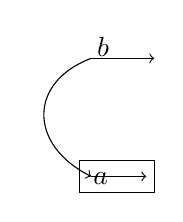
\begin{tikzpicture}[x=1cm,y=1cm]
\draw[->] (0,1.5)..controls(-.8,1.2)and(-.8,.4)..(0,0);
\draw[->] (0,1.5)--(.8,1.5);\draw[->] (0,0)--(.7,0);
\draw (-.15,-.2)rectangle(.8,.2);\node at (.15,1.65){$\unsure{b}$};\node at (.12,-.03){$\unsure{a}$};
\end{tikzpicture}}

c) Il existe une rigidification de $X$ invariante par $G$

\inserted{d) $(C,G)$ est isomorphe à la réalisation top. d'une op. de $G$ sur une carte combin.}

\inserted{Quand ces conditions sont remplies,}
\deleted{De plus,} l'espace des rigidifications de $X$ invariantes
par $G$ est contractile.

\[
a)\Longrightarrow b)\Longrightarrow c)\qquad\text{évident}
\]
\[
b)\Longrightarrow a)\quad\text{Revient à ceci:}
\]
\figure{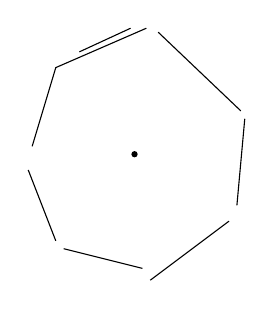
\begin{tikzpicture}[x=1cm,y=1cm]
\draw (-.8,.1)--(-.5,1.1)--(.65,1.6);
\draw (.8,1.55)--(1.85,.55);\draw(1.9,.45)--(1.8,-.65);
\draw(1.7,-.85)--(.7,-1.6);\draw(.6,-1.45)--(-.4,-1.2);
\draw(-.5,-1.1)--(-.85,-.2);\draw(-.2,1.3)--(.45,1.6);\fill(.5,0)circle(.04);
\end{tikzpicture}\quad
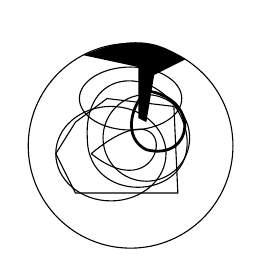
\begin{tikzpicture}[x=1cm,y=1cm]
\draw(0,0)circle(1.3);\fill(-.6,1.15)..controls(.2,1.5)and(.5,1.2)..(.7,1.1)--(.3,.9)--(.2,.3)--(.1,.35)--(.1,1)--cycle;
\draw (-.55,.1)..controls(-.6,1.1)and(.5,1)..(.7,.2)..controls(.9,-.7)and(-.55,-.8)..(-.55,.1);
\draw(-.7,.3)--(-.95,-.1)--(-.7,-.6)--(.6,-.6)--(.55,.5)--(-.3,.6)--(-.7,.3);
\draw(0,.6)ellipse(.65 and .4);\draw(-.25,-.1)ellipse(.7 and .6);\draw(.2,.1)circle(.55);\draw(-.5,-.1)..controls(.7,.9)and(.5,-.9)..(-.5,-.1);
\draw[line width=1pt](.2,.7)..controls(.9,.6)and(.8,-.2)..(.2,-.05)..controls(-.1,.1)and(0,.5)..(.2,.7);
\end{tikzpicture}}

Si un groupe \uline{fini}
opère \inserted{fid.} sur une carte, par
des opérations isotopes à id, il opère trivialt.
Ou encore: si un autom. d'ordre fini est
isotop. à id, \deleted{il opère tr.} c'est id. Il suffit de
le voir pour un disque fermé et un pt sur
le \inserted{bord du} disque -- on voit d'abord que c'est l'identité
sur le bord, \deleted{\unsure{par}} soit
\figure{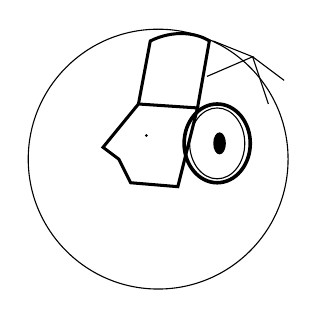
\begin{tikzpicture}[x=1cm,y=1cm]
\draw[thin](0,0)circle(1.65);
\draw[line width=1.1pt](-.7,.15)--(-.25,.7)--(.5,.65)--(.25,-.35)--(-.35,-.3)--(-.5,0)--cycle;
\draw[line width=1.1pt](-.25,.7)--(-.1,1.5)..controls(.2,1.65)and(.5,1.6)..(.65,1.5)--(.5,.65);
\draw(.7,1.5)--(1.2,1.3)--(.62,1.05);\draw(1.2,1.3)--(1.4,.7);\draw(1.2,1.3)--(1.6,1);
\draw[line width=1.3pt](.75,.2)ellipse(.42 and .5);\draw(.75,.2)ellipse(.35 and .45);\fill(.78,.2)ellipse(.08 and .14);\fill(-.15,.3)circle(.02);
\end{tikzpicture}\par
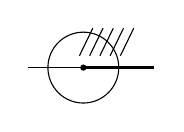
\begin{tikzpicture}[x=1cm,y=1cm]
\draw(0,0)circle(.45);\draw(-.7,0)--(.9,0);\draw[line width=1pt](0,0)--(.9,0);\fill(0,0)circle(.04);
\foreach \x in {-.05,.08,.21,.34,.47}{\draw[thin](\x,.15)--(\x+.17,.5);}
\end{tikzpicture}}
